\def\year{2015}
\documentclass[letterpaper]{article}
\usepackage{aaai}
\usepackage{color}
\usepackage{courier}
\usepackage{enumerate}
\usepackage{graphicx}
\usepackage{helvet}
\usepackage{multirow}
\usepackage{outline}
\usepackage{siunitx}
\usepackage{subfigure}
\usepackage{times}
\usepackage{url}
\usepackage{amsmath}
\usepackage{booktabs}

\newcommand{\beq}{\begin{equation}}
\newcommand{\eeq}{\end{equation}}
\newcommand{\citenoun}[1]{{\citeauthor{#1} \shortcite{#1}}}
\newcommand{\cut}[1]{}
\newcommand{\fixme}[1]{{\color{blue}\textless #1 \textgreater}}
\newcommand{\voc}[1]{{\sl #1}}
\newcommand{\y}{\mathbf{y}}

\nocopyright
\frenchspacing
\setlength{\pdfpagewidth}{8.5in}
\setlength{\pdfpageheight}{11in}
\pdfinfo{
/Title ()
/Author (Virgile Landeiro Dos Reis, Aron Culotta)}
\setcounter{secnumdepth}{2}  
 \begin{document}
% The file aaai.sty is the style file for AAAI Press 
% proceedings, working notes, and technical reports.
%
\title{}
\author{
Virgile Landeiro Dos Reis \and Aron Culotta\\
Department of Computer Science\\
Illinois Institute of Technology\\
Chicago, IL 60616\\
vlandeir@hawk.iit.edu, aculotta@iit.edu\\
}
\maketitle

% Outline
\cut{

Overall research question:
- can we find significant differences in the food consumption of people who exercise vs people who don't exercise using matched samples on twitter data?

Research questions:
  - can we find interesting differences in the food-related vocabulary used by people who exercise vs. people who don't? what are the most predictive words for each class once data is reduced to food-related tweets?
  - can we find significant differences in the network of users that exercise vs users who don't?

Related Work: social media + nutrition, social media + food deserts
  - health:
  - food: weber paper + de choudhury paper on instagram food deserts

Data:
  - sporty twitter data
  - filter with foodb + weber keywords
  - compute score using wordnet while removing ambiguous words

Methods:
  - text level: compare most predictive features for each class, compare most referenced food categories using weber dataset.
  - network level: compare number of friends that are known to be health related (food brands + health related twitter accounts).
}

\begin{abstract}
\begin{quote}
  
\end{quote}
\end{abstract}

\section{Introduction}

\section{Related Work}

\section{Data}

\subsection{Physically active users}

\cut {
  - landeiro2015using data
  - explain how it has been built: hashtag of tracking apps gives us the physically active users. matching on social media features, gender, and location gives us the control group.
}

We use the dataset from \cite{landeiro2015using} as our main dataset. This dataset is composed of two groups of users: a group of physically active users, and a group of users who do not exercise. We summarize in a few points how this dataset has been constructed:

\begin{enumerate}
  
  \item To detect physically active users, \citeauthor{landeiro2015using}
  leveraged existing physical activity tracking applications such as Nike Plus,
  Runtastic, or RunKeeper. These applications help active users track their
  progress and give them a summary of their workouts. Additionally, it can
  automatically tweet a summary of each workout associated with a dedicated
  hashtag if the user has activated this function. When a user is found to have
  used one of these dedicated hashtags, it is placed in the treatment group.

  \item To build the control group, \citeauthor{landeiro2015using} used a
  technique where each user in the treatment group is matched with another user.
  To find this match for a user $i$, they first collected the list of accounts
  $F_i$ that have a mutual-follow relationship with $i$ on Twitter. Then, they
  filtered out from $F_i$ users that were not of the same gender than $i$ (using
  the US Census data) and users that were not in the same city or same state as
  $i$ (using heuristics on the Twitter location field of each user). Finally,
  they built a cosine similarity score between $i$ and the remaining users in
  $F_i$ on social media features (number of followers, number of followees,
  number of posts) and kept the user in $F_i$ with the highest score as the best
  match to be included in the control group.

  \item For each of the 2,322 users in this dataset (1161 in each group), they
  collected the most recent tweets, up to 3,200.

\end{enumerate}

\subsection{Food-related datasets}

Because the Twitter dataset built in the previous section does not focus on food tweets, we merge three datasets with food information into one in order to construct a large dataset of food vocabulary.

\begin{enumerate}

  \item FooDB\footnote{http://foodb.ca/} is an ensemble of resources on food
  constituents, chemistry and biology. In particular, we use the dataset listing
  889 food sources associated with a category (e.g. kiwi is associated with the
  fruits category and turkey is in the poultry category).

  \item In \cite{abbar2015you}, the authors combined a large data collection of
  50M tweets on manually selected keywords, bootstraping techniques, and
  crowdsourcing to build a dataset of food vocabulary of 461 words with the
  category they belong to as well as the average amount of calorie per serving
  for each food.

  \item Finally, we use WordNet \cite{miller1995wordnet}, the popular lexical
  database for English, and we build a dynamic programming algorithm that looks
  up the ancestors of a word up to the tree root and returns True if at least one ancestor is one of:
  \begin{itemize}

    \item food: any substance that can be metabolized by an animal to give
    energy and build tissue.
    
    \item food: any solid substance (as opposed to liquid) that is used as a
    source of nourishment.

    \item edible nut: a hard-shelled seed consisting of an edible kernel or meat
    enclosed in a woody or leathery shell.

  \end{itemize}

\end{enumerate}

\cut{
  - foodb: http://foodb.ca/
  - wordnet: miller1995wordnet
  - you tweet what you eat
}

\subsection{Exemplar health Twitter accounts}

Using a subset of the data built in \cite{culotta2016mining}, we obtain a list
of 407 accounts that tweet about health, called exemplar accounts. These
exemplar accounts are collected using Twitter Lists (i.e. manual aggregation of
accounts). First, a query (e.g. "health") is sent to Twitter's search engine,
which returns Twitter Lists and tweets. If an account appear in at least two of
the top 50 Lists, then this account becomes an exemplar account for the given
query.

\section{Experiments and results}

To evaluate the differences in the relation to food and health between users who exercise and users who do not exercise, we experimented at two levels. First, we looked at the distribution of food-related words in both groups and studied the most discriminative features between both groups after keeping a subset of users that we detected tweeted about food. Then, we focused on a network-level analysis where we compared the relation that the users in our treatment and control groups have with health exemplar accounts.


\subsection{Text-level analysis}

To evaluate the vocabulary differences between our two groups of users, we started by filtering out tweets that are not about food. We then trained two models: one to underline the most predictive features of each group (linear SVM), and one to explain similar observations and group them together (Latent Dirichlet Allocation).

\subsubsection{Filter food-related tweets}

In order to remove irrelevant tweets for our analysis, we started by combining
the FooDB dataset and the food sources in the dataset developed by
\citeauthor{abbar2015you}. In later steps, we noticed that some food words were
more often associated with non food-related topics. For example, the word
"apple" was more frequently used in reference to the technology company
\verb+Apple+ and its products than it was to reference the actual fruit. For
this reason, we manually created a set of excluded words that we detect as being
sources of false positive in the detection of food-related tweets. Initially,
this set is composed of the words \verb+apple+ (the tech company),
\verb+raspberry+ (the \$30 computer raspberry pi), \verb+blackberry+ (the
smartphone company), \verb+kevin+ (Kevin Bacon), as well as the words displayed
in Table~\ref{tab:excluded-words}. We will see in some of the next steps that we
had to come back to this step and add words to the list of excluded words in
order to remove more false positive tweets.

\begin{table}
  \center
  \begin{tabular}{lllllllll}
  \toprule
   bite &  bootleg &     brain &  buffalo &       cat \\
  enter &   centre &  coloring &      cup &       cut \\
   date &      dip &      dish &      dog &      feed \\
   game &    green &      jack &    joint &    kisses \\
    leg &     must &       pop &    punch &      rock \\
   rose &  scratch &  shoulder &     side &  snowball \\
  stick &    stock &    sucker &    table &     white \\
  \bottomrule
  \end{tabular}
  \label{tab:excluded-words}
  \caption{Example of words detected as food-related that we manually remove from our analysis.}
\end{table}

We end up with a list of 1,217 food-related words $food\_list$, and a list of words
inclined to yield false positive tweets $excluded\_list$. Then, for each tweet $t$ of each user, we keep $t$ if none of the words in $t$ are in $excluded\_list$ and if at least one of the words in $t$ is in $food\_list$.

\subsubsection{Filter food-conscious users}

Once we obtained the food-related tweets for each user in both groups, we
compute a score for each tweet $t$ as the proportion of terms that are
food-related (i.e. number of food terms in $t$ over the total number of terms).

In order to define if a term is a food term, we not only use $food\_list$ and
$excluded\_list$ as in the previous step, but we also make use of our algorithm
based on WordNet. This allows us to detect a wider range of food terms to
compute the score for users. We decided not to use the WordNet-based algorithm
in the previous step to avoid detecting too many false positive food-related
tweets. Indeed, with our algorithm, all the words that have at least one
ancestor being "food"" or "edible nut" in the WordNet graph will be classified
as food-related terms. Therefore, a large amount of words that have several
meanings and for which the main meaning is not related to food will be
classified as food-related (e.g. "must" is a kind of freshly pressed grape
juice, "dog" is a way to describe a "hotdog").

Finally, we keep a physically active user $u$ in our treatment group if $u$ and
its match in the control group have at least 15 food-related tweets with a score
of .15 or more. This yields 530 users that are talking about food in each group.

\subsubsection{Most predictive features for each group}

Using the food-related tweets of each of the remaining 1060 users, we analyze
the differences between the most predictive features of the physically active
group and the most predictive features of the matched group. To do so, we create
a features vector for each user by removing retweets, tokenizing the remaining
tweets using unigrams, removing punctuation signs as well as stopwords. Then, we
fit a linear SVM model on these features where the label of each user is the
group to which it belongs. In table~\ref{tab:top_fts_all}, we report the twenty most important features for each class.

\begin{table}
  \center
\begin{tabular}{lp{0.3\textwidth}}
\toprule
\textbf{Control}  &  last, wish, right, girl, dr, king, celery, plus, real, thanksgiving, hate, corner, lost, gin, wrong, episode, event, ah, smoked, mozzarella \\
\textbf{Treatment} & others, state, looks, burrito, starbucks, used, cookies, co, cafe, pic, run, man, drinking, lots, NUMBERk, pub, day, broccoli, going, grill \\
\bottomrule
\end{tabular}
  \label{tab:top_fts_all}
  \caption{20 most predictive features for each group.}
\end{table}

\begin{table}
\center
\begin{tabular}{llll}
\toprule
\textbf{Control} & & \textbf{Treatment} & \\
Rank & Feature & Rank & Feature \\
\cmidrule(lr){1-2} \cmidrule(lr){3-4}
7  &      celery & 4  &    burrito \\
14 &         gin & 7  &    cookies \\
20 &  mozzarella & 18 &   broccoli \\
21 &     pickles & 23 &    caramel \\
34 &        deer & 25 &  breakfast \\
40 &    molasses & 30 &     carrot \\
43 &     bananas & 31 &   burritos \\
50 &        wrap & 32 &    coconut \\
57 &       curds & 33 &     onions \\
62 &       frank & 34 &     citrus \\
\bottomrule
\end{tabular}
\end{table}

\subsubsection{Differences in food categories between groups}

\begin{figure}
  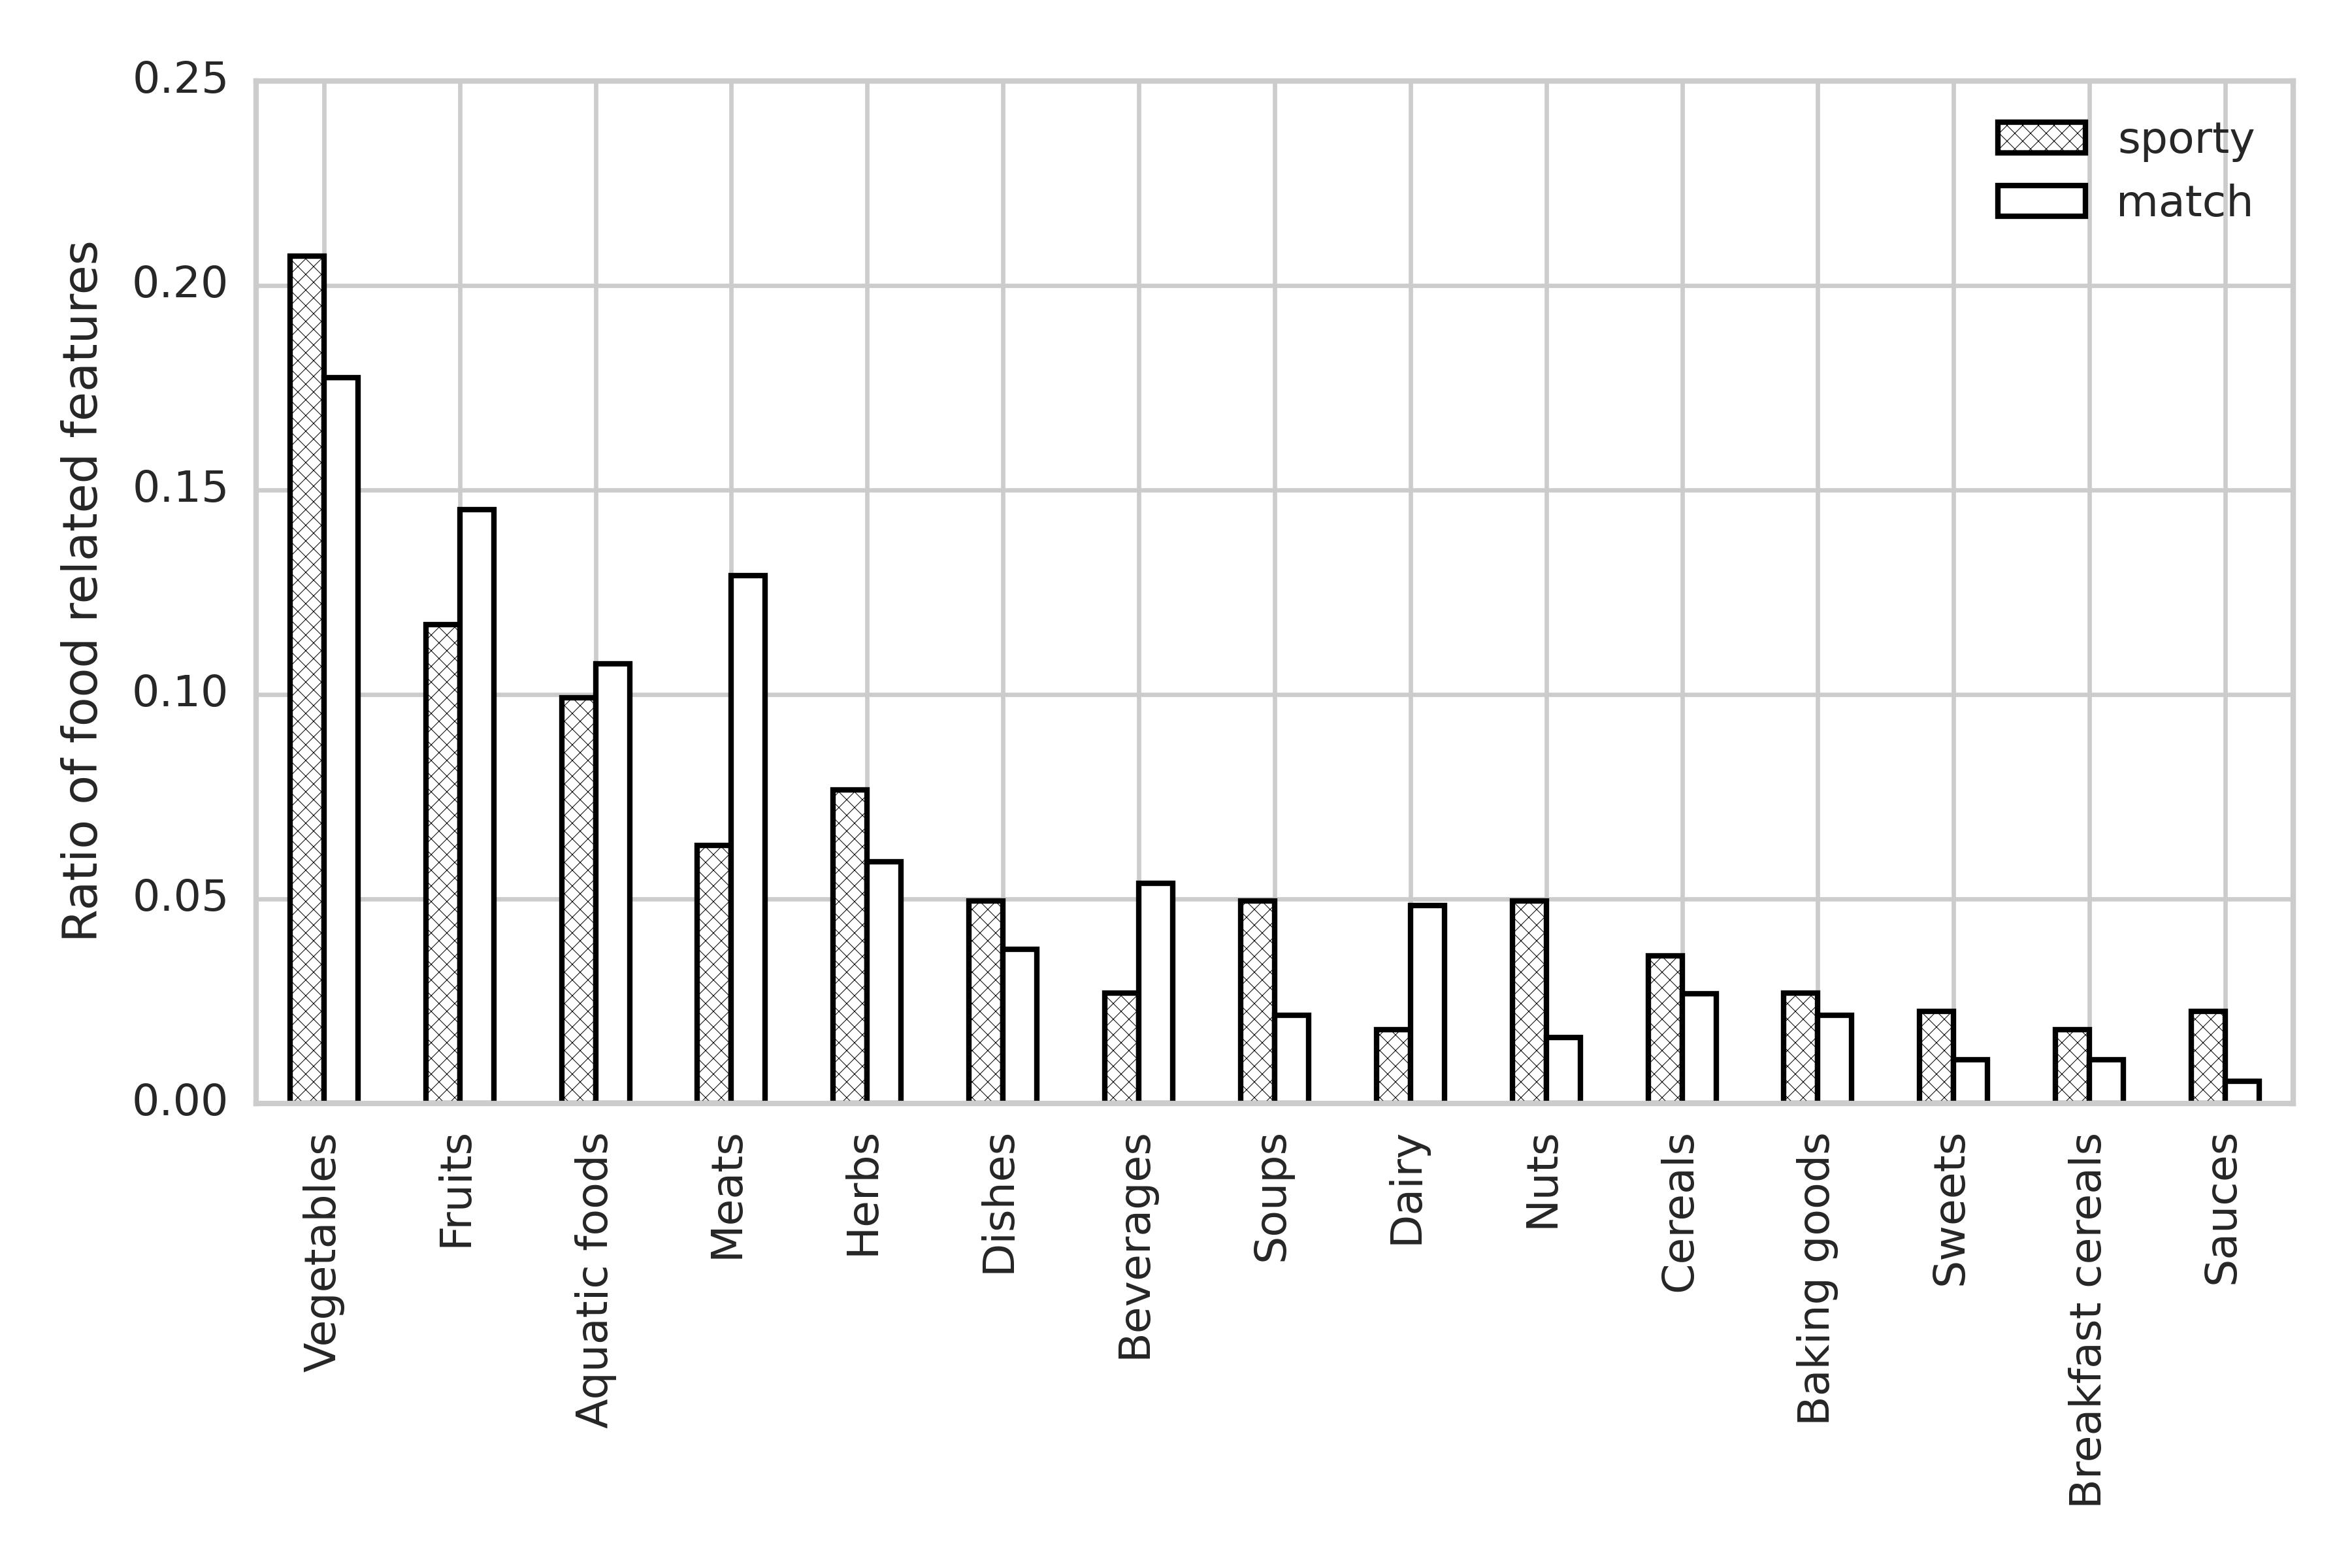
\includegraphics[width=.45\textwidth]{figs/top_food_cats.png}\\
  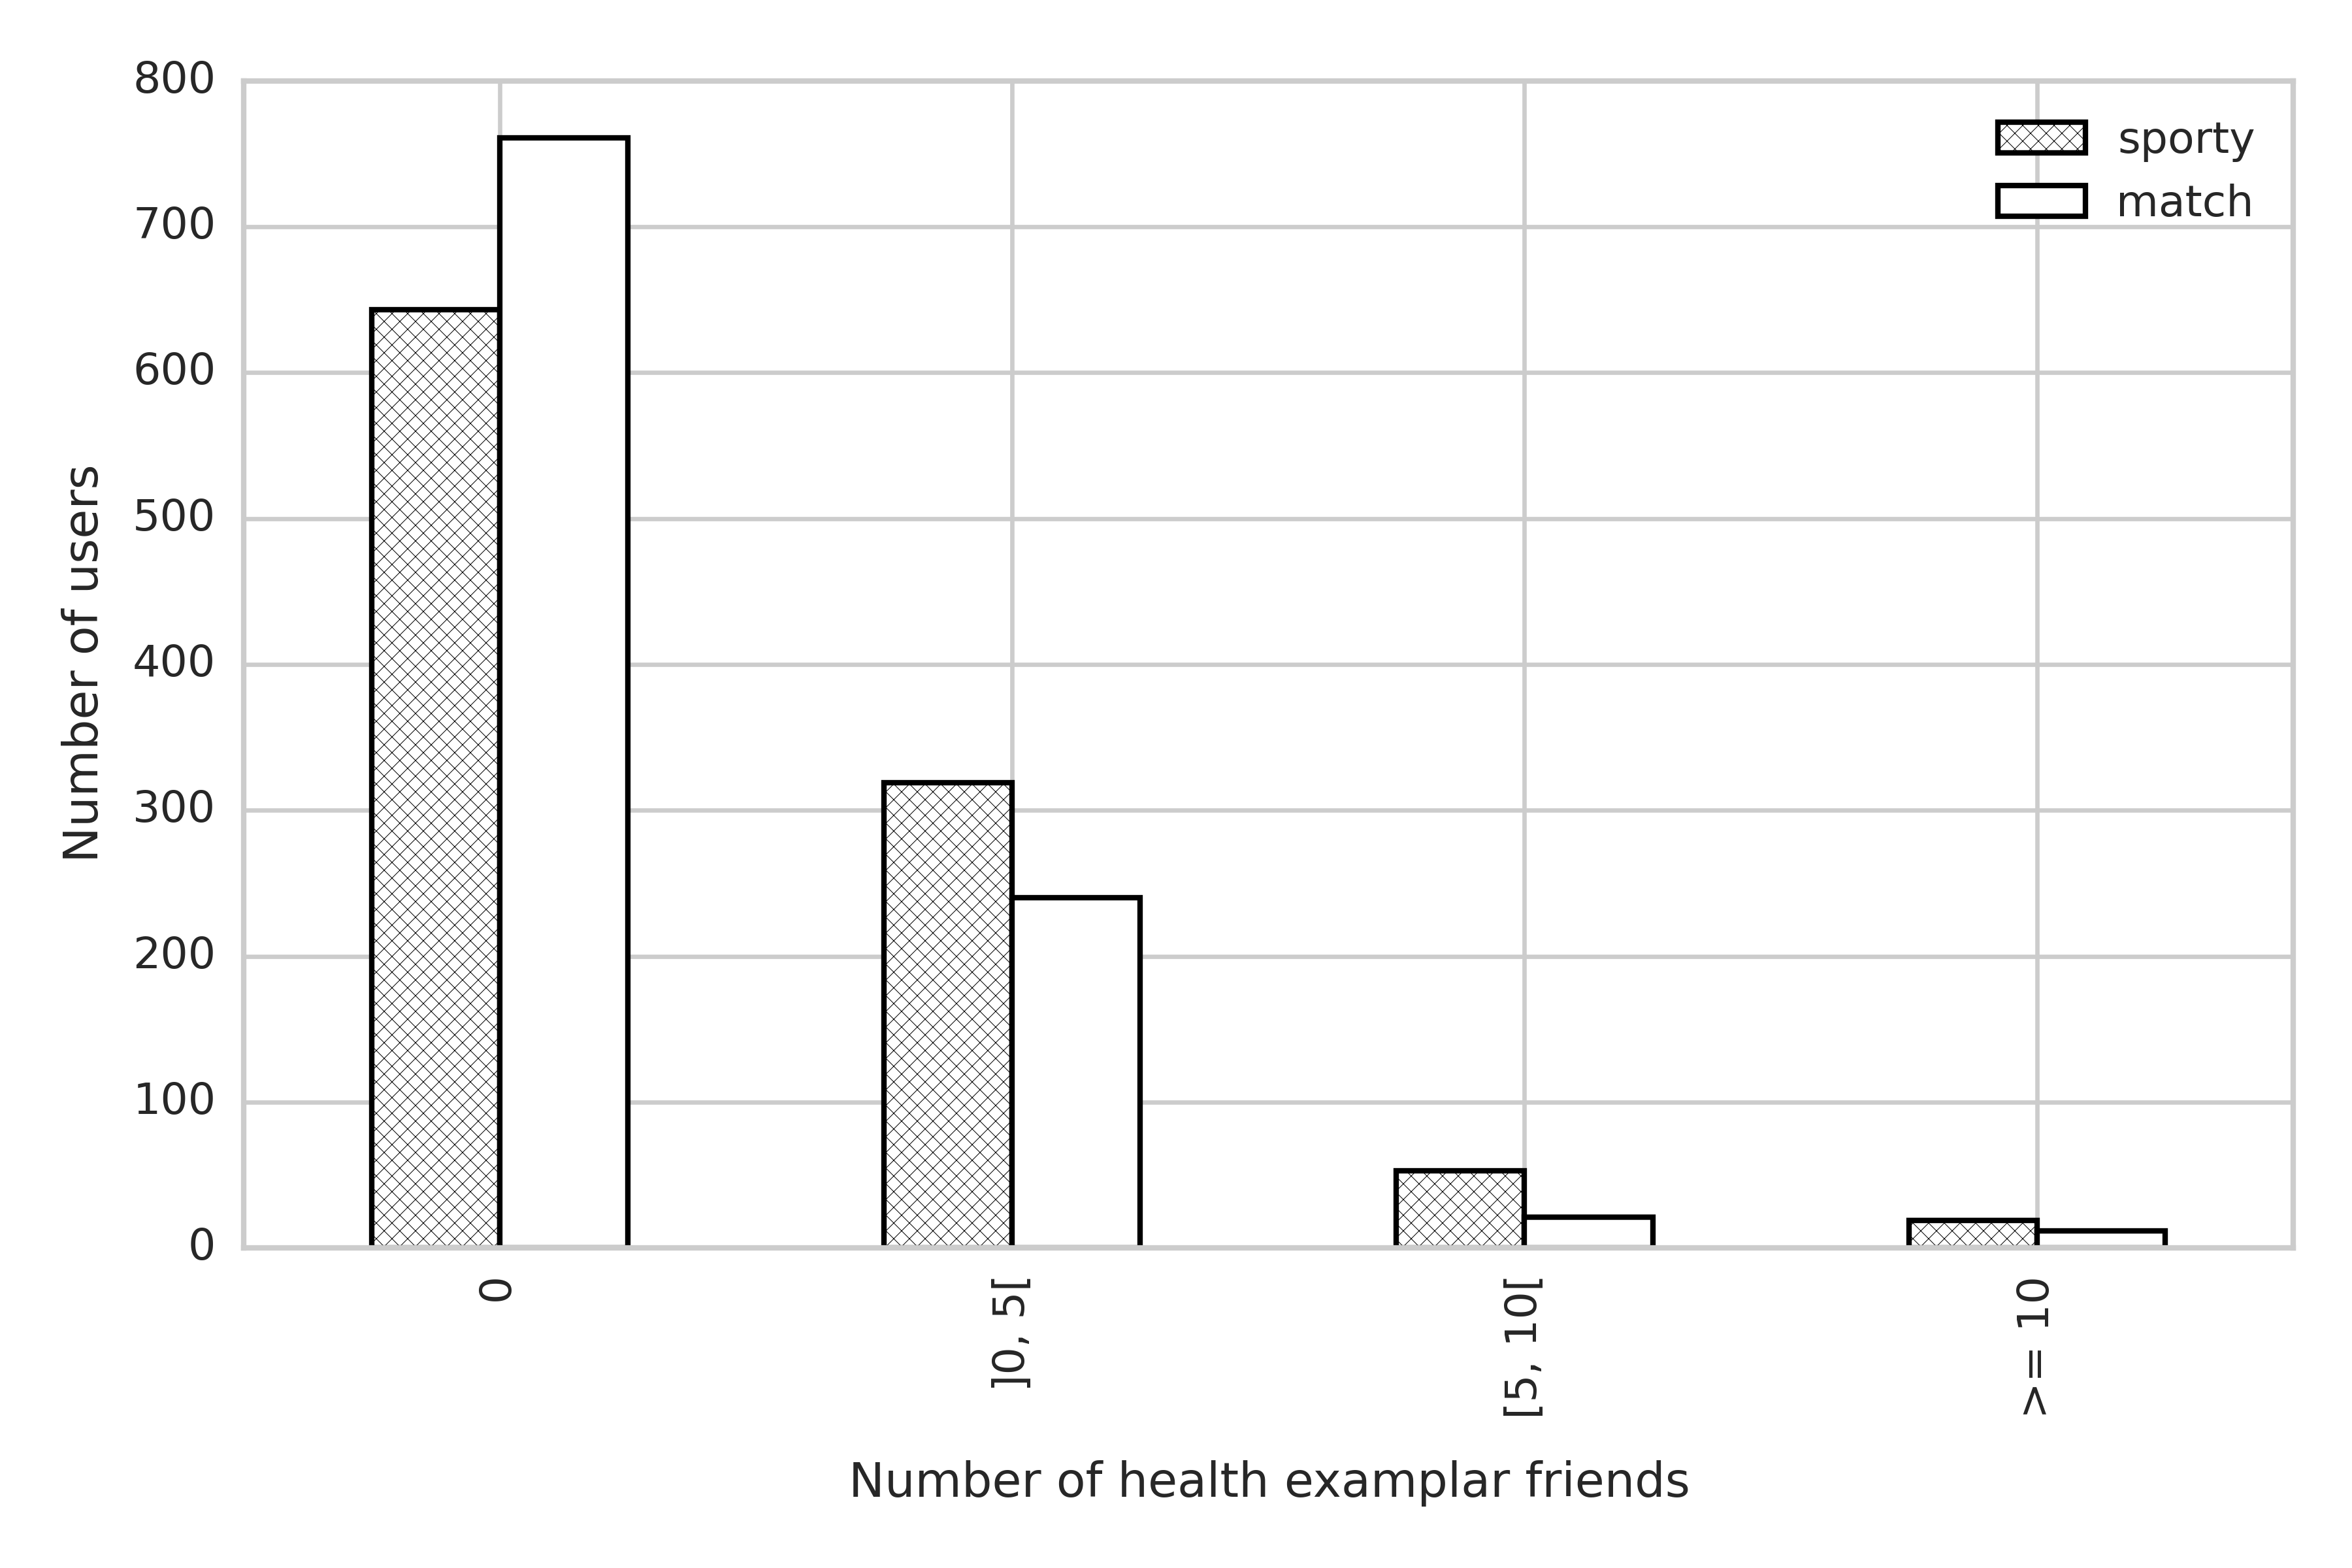
\includegraphics[width=.45\textwidth]{figs/exemplar_friends.png}\\
  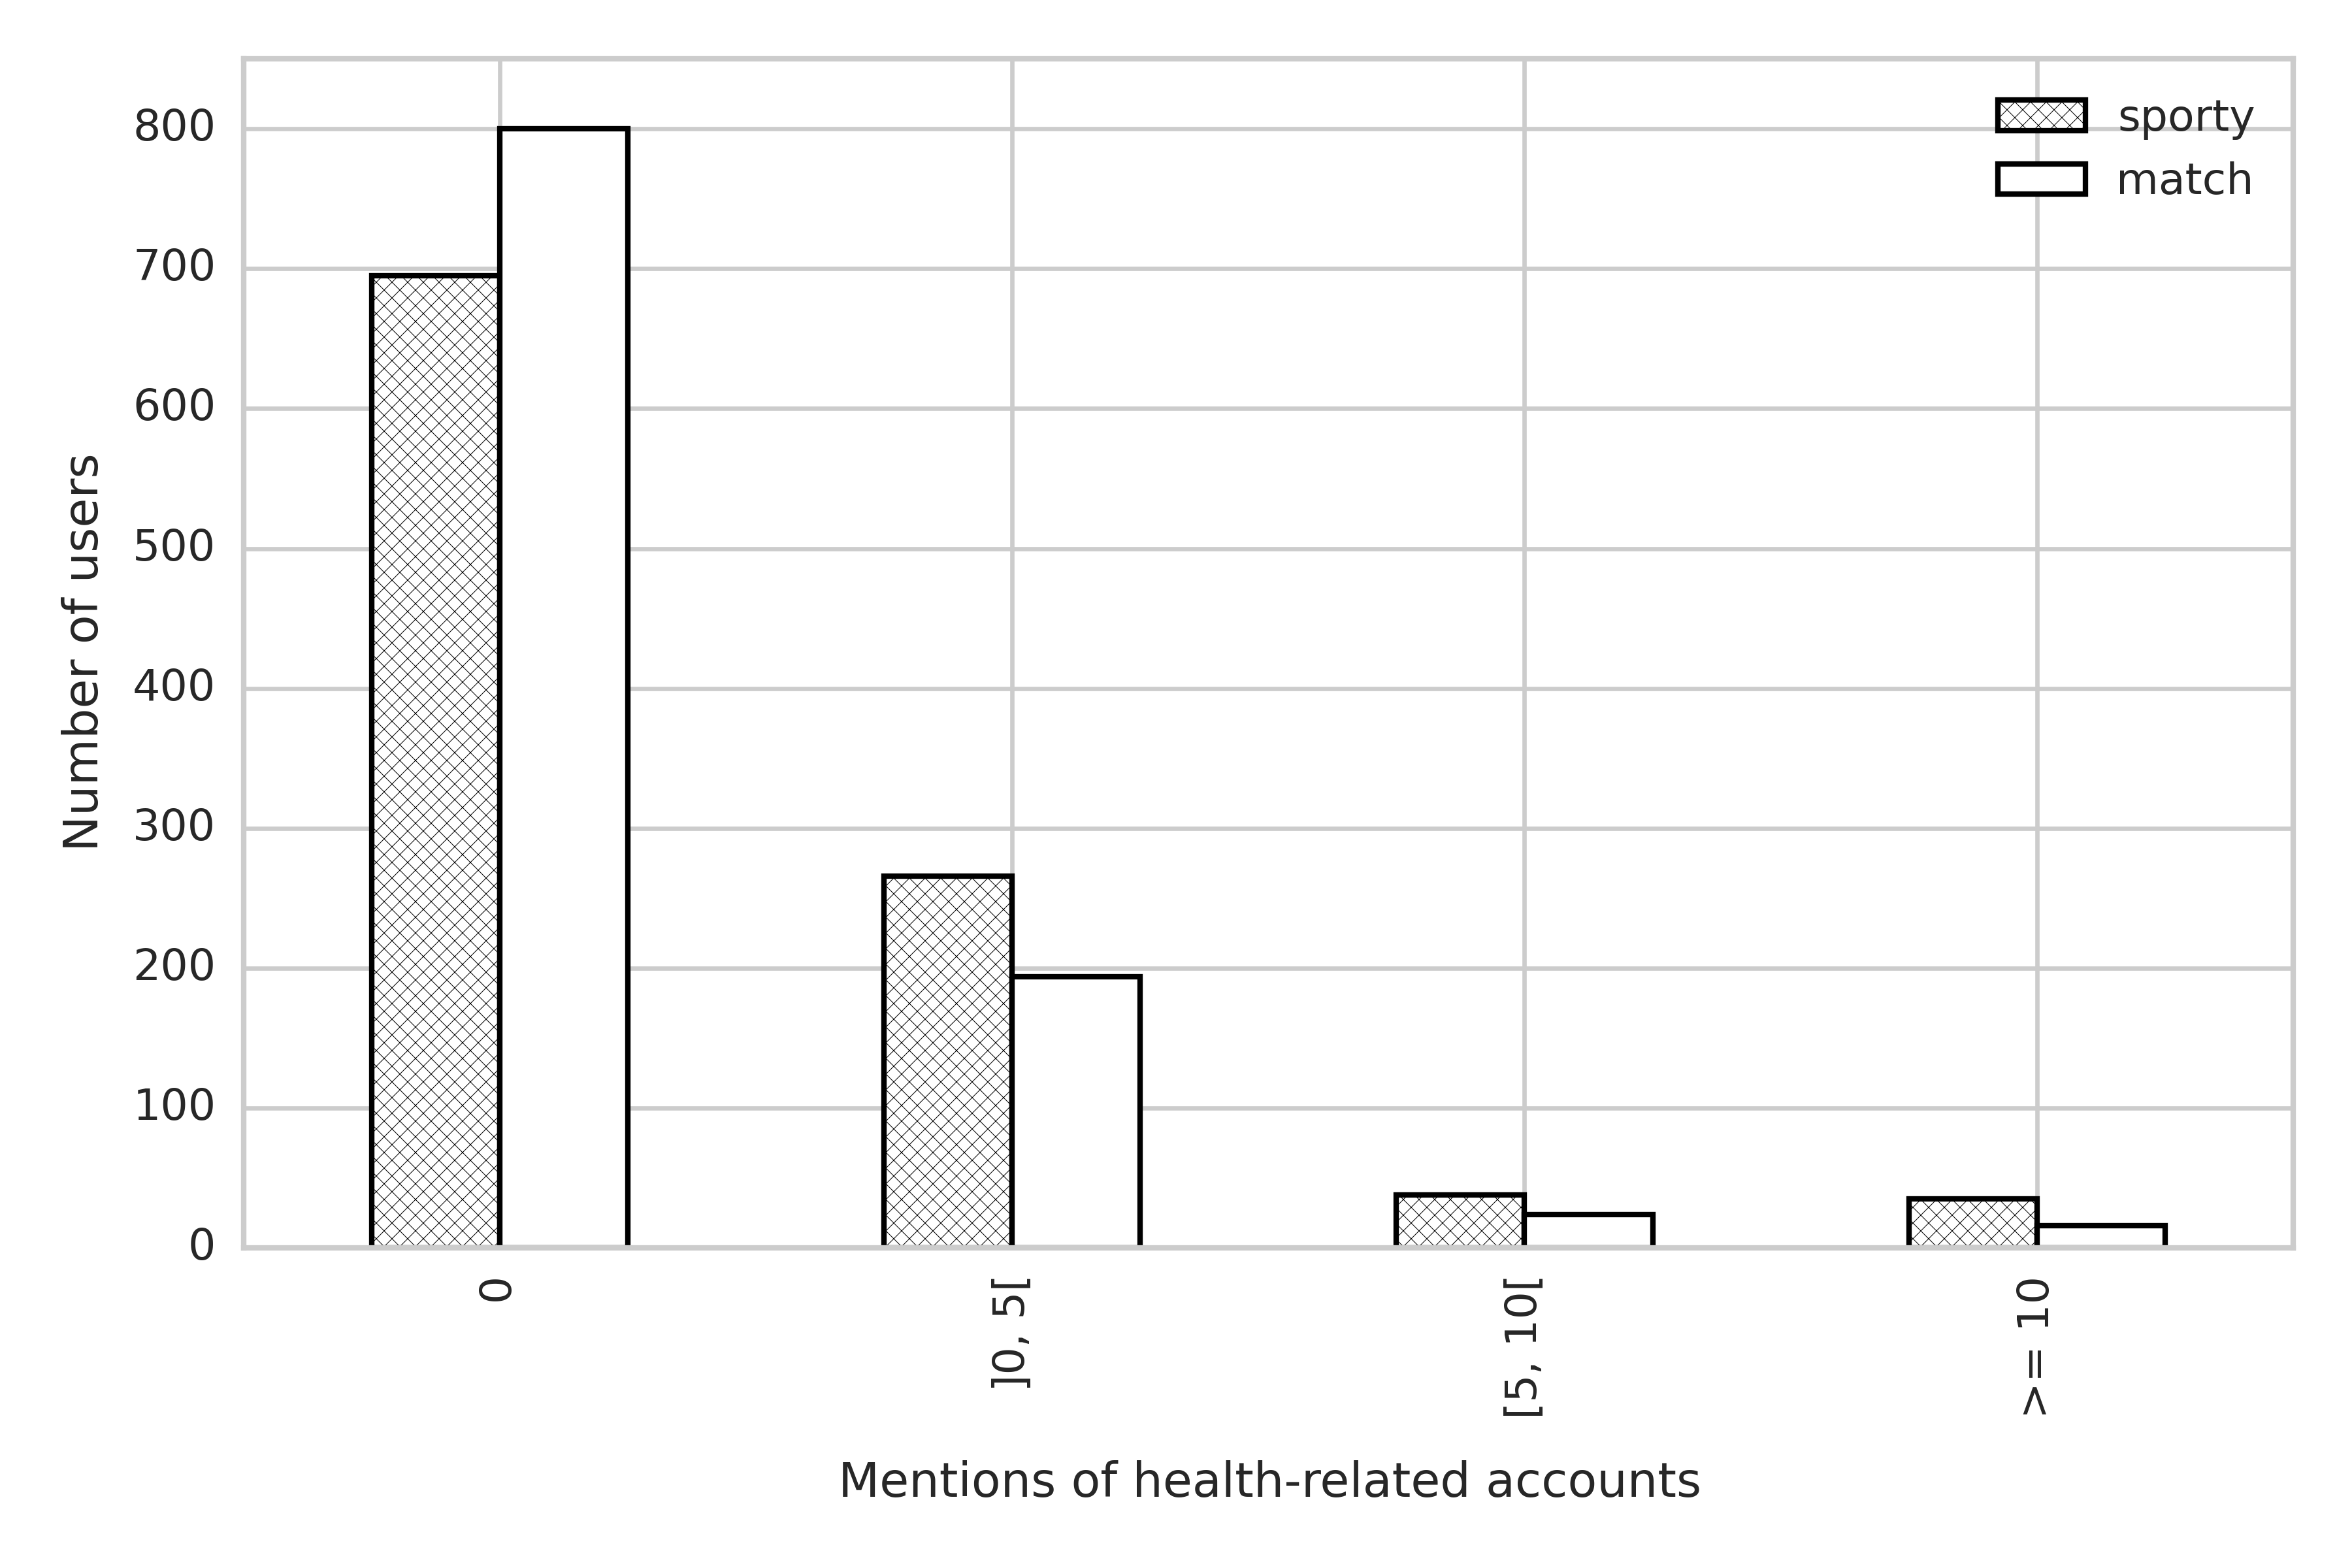
\includegraphics[width=.45\textwidth]{figs/exemplar_mentions.png}\\
\end{figure}

\subsection{Network-level analysis}

\subsubsection{Follow relationship}

\subsubsection{Mention relationship}

\section{Discussion}

\bibliographystyle{aaai}
\bibliography{sporty}
\end{document}
